% Preamble
\documentclass[../Relazione_circuiti]{subfiles}

% Packages

\graphicspath{{\subfix{../images/}}}

% Document
\begin{document}

\subsection{Analisi preliminare qualitativa}

\begin{figure}[H]
\centering

\begin{subfigure}[b]{0.3\textwidth}
\centering
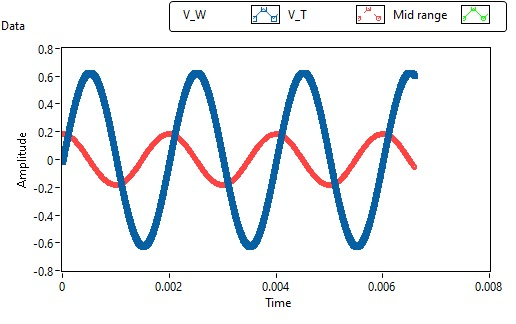
\includegraphics[width=\textwidth]{Cross_waveform_500.jpeg}

\caption{Segnali a 500Hz}
\label{fig:signal_500}

\end{subfigure}

\hfill

\begin{subfigure}[b]{0.3\textwidth}
\centering
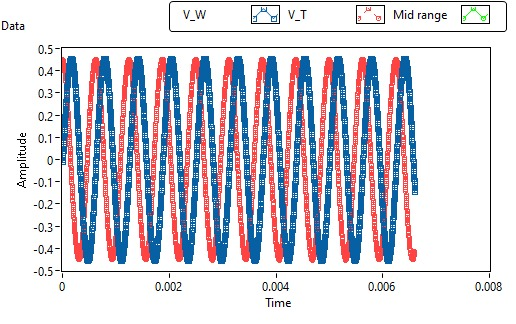
\includegraphics[width=\textwidth]{Cross_waveform_1600.jpeg}

\caption{Segnali a 1600Hz}
\label{fig:signal_1600}

\end{subfigure}

\hfill

\begin{subfigure}[b]{0.3\textwidth}
\centering
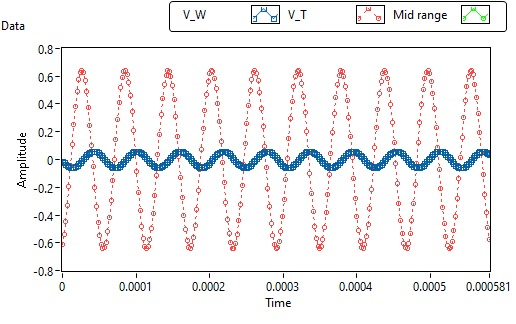
\includegraphics[width=\textwidth]{Cross_waveform_17000.jpeg}

\caption{Segnali a 17kHz}
\label{fig:signal_17k}

\end{subfigure}

\caption{Segnali osservati sui rami Woofer (blu) e Tweeter (rosso) a frequenza fissata. Le incertezze non sono visibili a causa della scala.}
\label{fig:signal_waveforms}

\end{figure}

La figura \ref{fig:signal_waveforms} mostra la forma d'onda dei segnali osservati sui rami Woofer e Tweeter in risposta ad un segnale sinusoidale. La figura \ref{fig:signal_1600} mostra il comportamento nei pressi della frequenza di cross attesa, la figura \ref{fig:signal_500} a 1/3 e la figura \ref{fig:signal_17k} a circa 10 volte.

Si osserva (Figura \ref{fig:signal_1600}) che, coerentemente con quanto atteso, i segnali hanno ampiezza simile nei pressi di $f_{cross}$. A basse frequenze si osserva (Figura \ref{fig:signal_500}) un'attenuazione del 60\% dell'ampiezza sul ramo Tweeter e nessuna alterazione sul Woofer, ad alte frequenze un'attenuazione sul Woofer dell'86\% e nessuna sul Tweeter (Figura \ref{fig:signal_17k}).


\subsection{Analisi della frequenza misurata}

\subsection{Analisi dell'ampiezza}

\subsection{Analisi della fase}

\begin{figure}[H]
\centering

\begin{subfigure}{=0.5\textwidth}
\centering
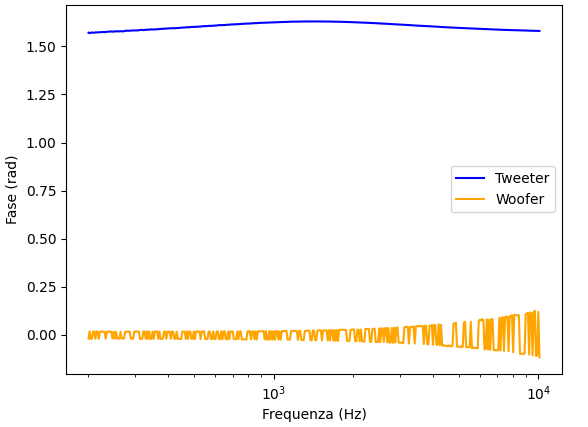
\includegraphics[width=12cm]{phase_dataonly.png}

\caption{Sfasamento Tweeter-Woofer. La frequenza è in scala logaritmica. Le incertezze non sono visibili a causa della scala.}
\label{fig: pdiff_dataonly}

\end{subfigure}

\begin{subfigure}{=0.5\textwidth}
\centering
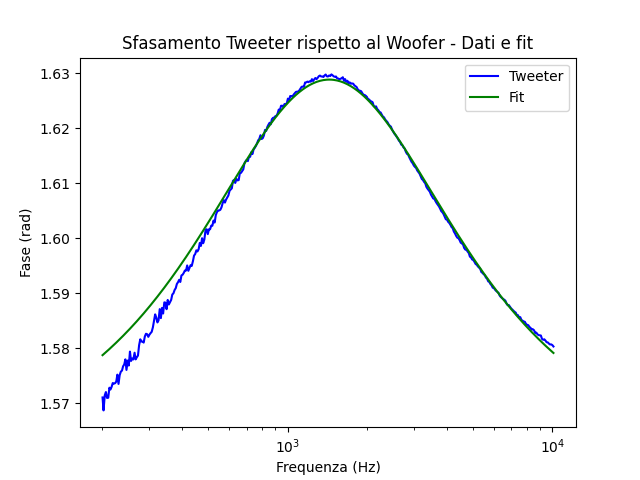
\includegraphics[width=12cm]{phase_cross.png}

\caption{Sfasamento Tweeter-Woofer e sovrapposizione con fit. La frequenza è in scala logaritmica. Le incertezze non sono visibili a causa della scala.}
\label{fig: pdiff_fit_data}

\end{subfigure}

\end{figure}




\end{document}